\chapter{Graphs}
\label{app:cytoscape}

\begin{figure}[ht]
  \centering
  \includegraphics[width=\linewidth]{DegPatch2.pdf}
  \caption{Patch Delineated by 2 Degrees of Socio-Technical Separation}
  \label{fig:degpatch2}
\end{figure}
\begin{figure}[ht]
  \centering
  \includegraphics[width=\linewidth]{DegPatch3.pdf}
  \caption{Patch Delineated by 3 Degrees of Socio-Technical Separation}
  \label{fig:degpatch3}
\end{figure}
\begin{figure}[ht]
  \centering
  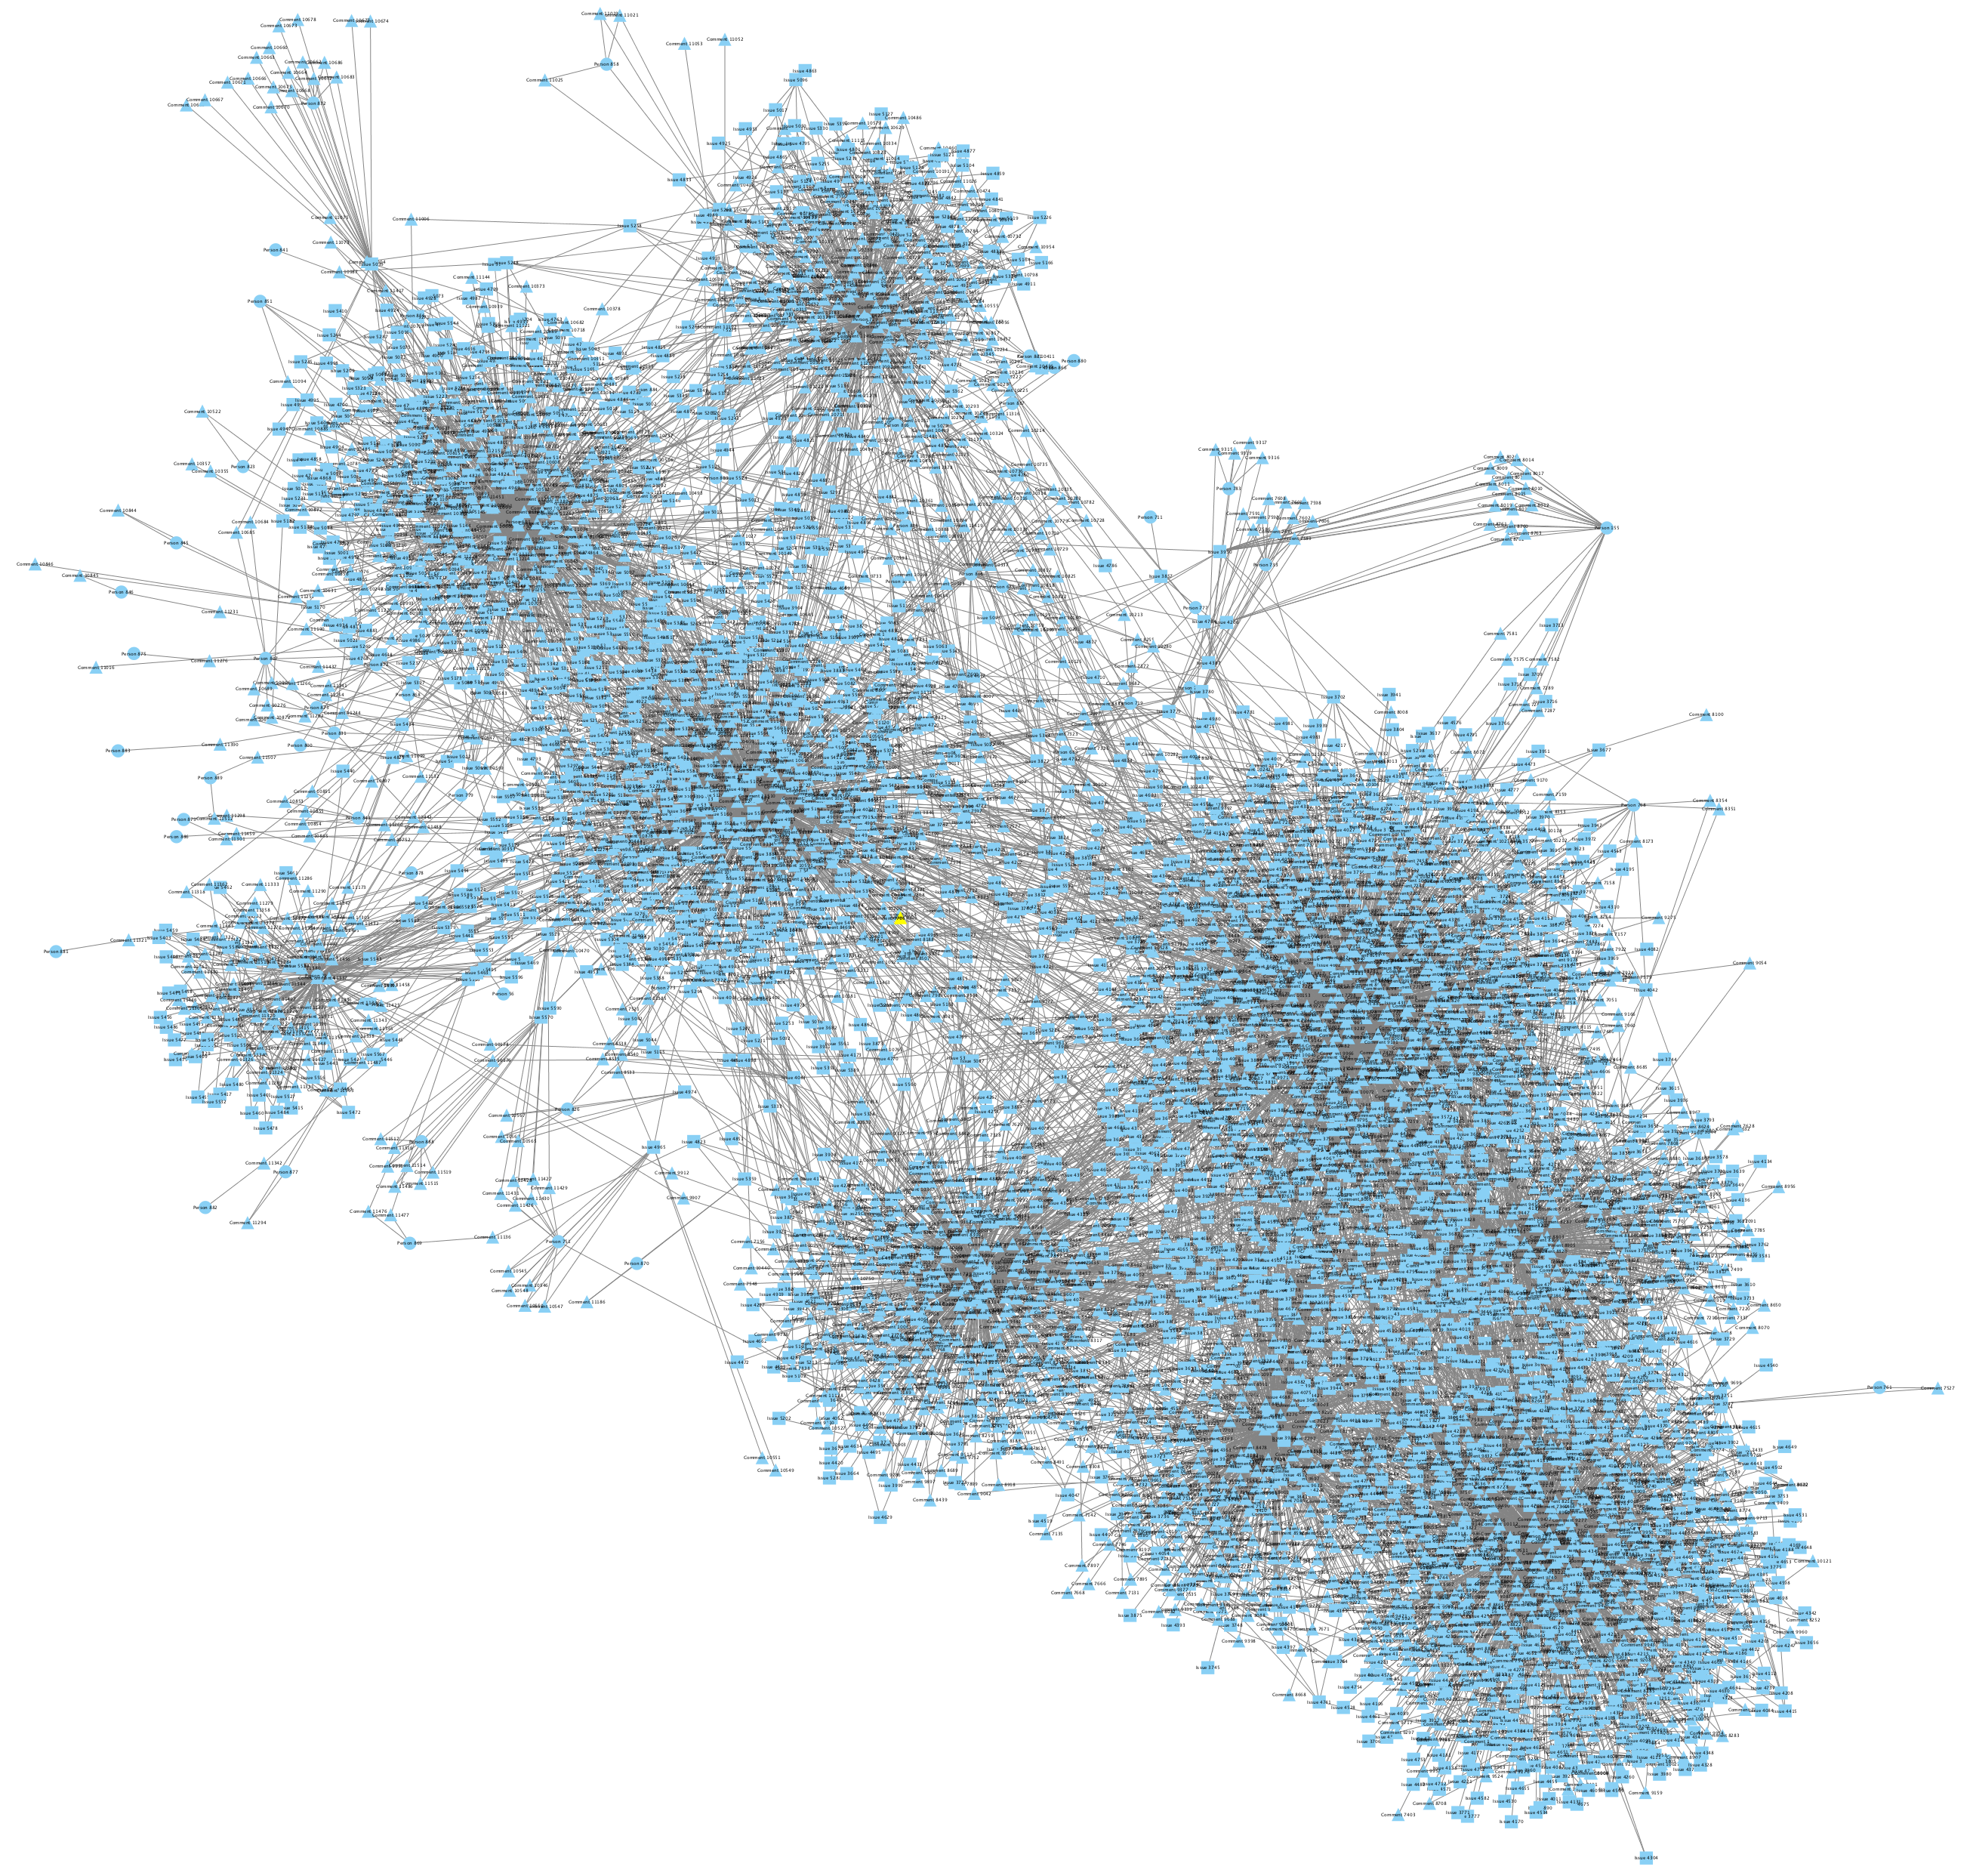
\includegraphics[width=\linewidth]{DegPatch4.pdf}
  \caption{Patch Delineated by 4 Degrees of Socio-Technical Separation}
  \label{fig:degpatch4}
\end{figure}
% \begin{figure}[ht]
%   \centering
%   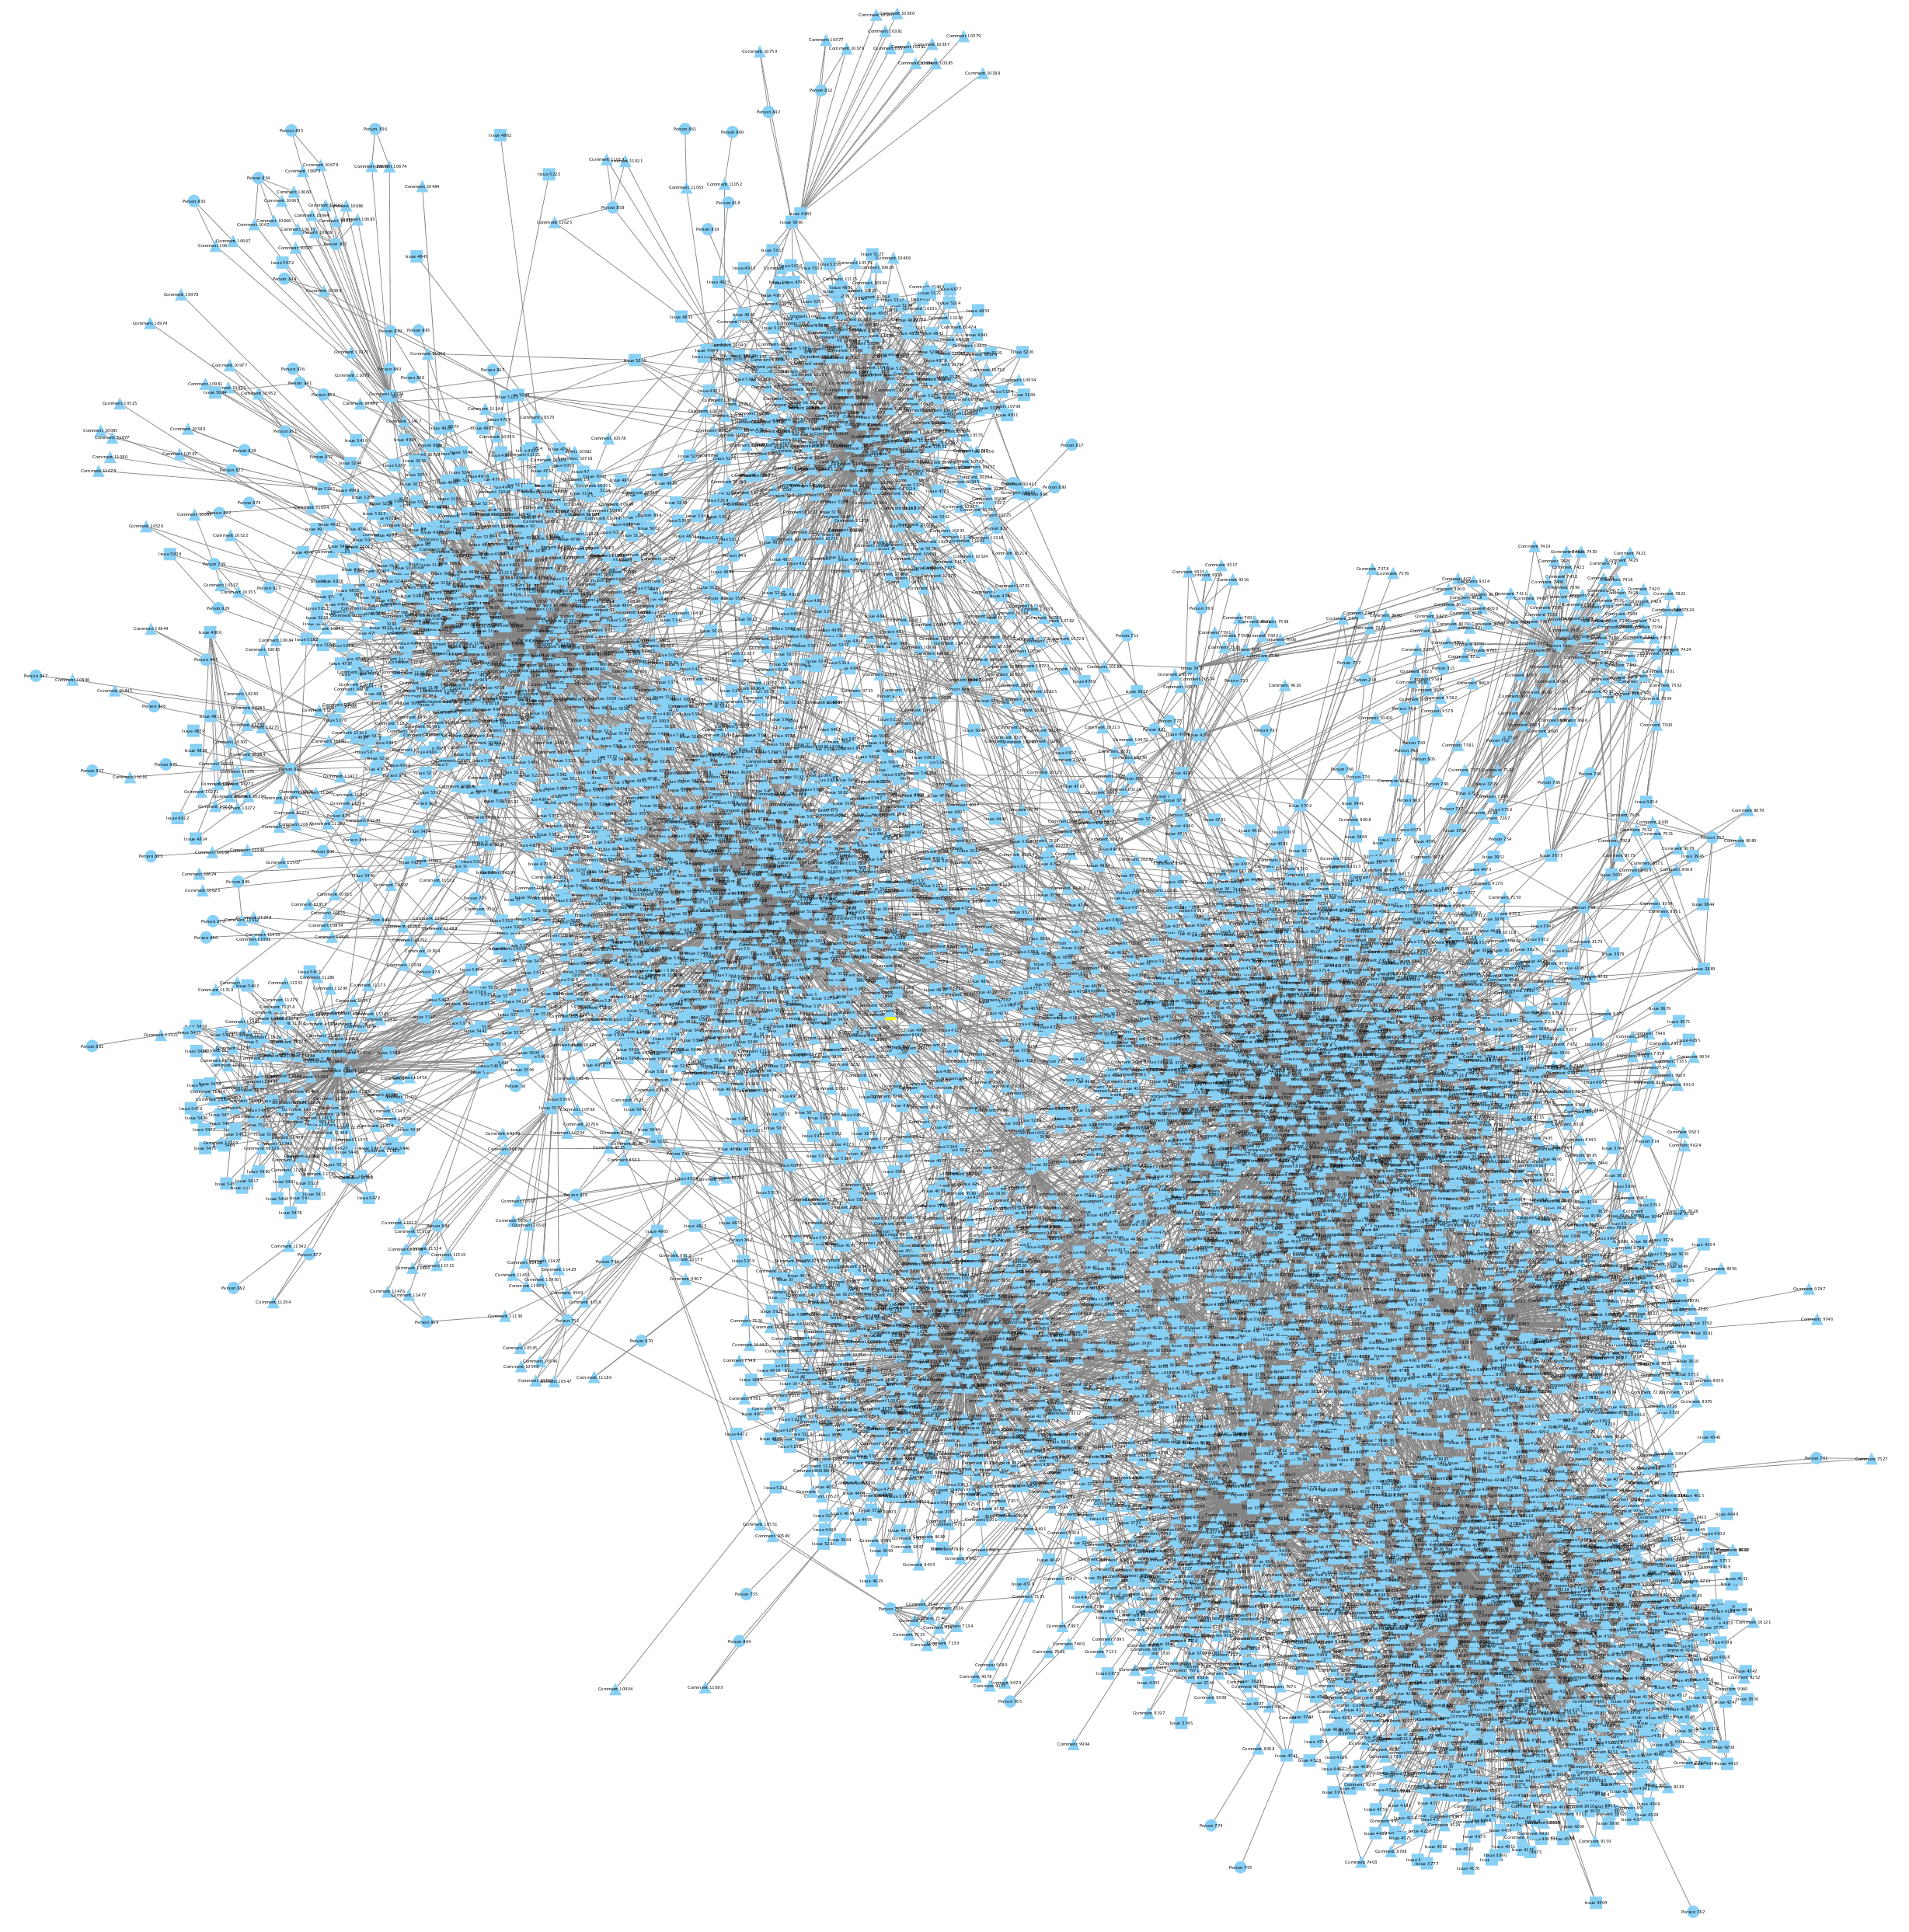
\includegraphics[width=\linewidth]{DegPatch5.pdf}
%   \caption{Patch Delineated by 5 Degrees of Socio-Technical Separation}
%   \label{fig:degpatch5}
% \end{figure}

\begin{figure}[ht]
	\centering
	\includegraphics[width=\linewidth]{c9396weight.png}
	\caption{Example Cytoscape Visualization of Project With Spreading Activation Applied. Darker Nodes Have Higher Activation}
	\label{fig:c9396}
\end{figure}

% \chapter{Jira Examples}
% \label{app:jira}

% \section{Complete DASHBUILDER Answer Set}
% DASHBUILDER was the shortest answer set of our four projects, consisting of 18 Question/Answer pairs. The original answer sets included more columns, including ones that provided evidence of answers. The table below omits these columns, as they weren't used for our script.

% \csvreader[tabular=|l|l|c|l|l|,
%     table head=\hline Body & Asker & Answered & By & Notes \\\hline,
%     late after line=\\\hline]%
% {images/dashbuilder.csv}{Body=\Body,Asker=\Asker,Answered=\Answered,By=\By,Notes=\Notes}%

\chapter{Code}
\label{app:python}

\lstset{ 
  basicstyle=\tiny,                % the size of the fonts that are used for the code
  breaklines=false,                % sets automatic line breaking
  captionpos=b,                    % sets the caption-position to bottom
  keepspaces=true,                 % keeps spaces in text, useful for keeping indentation of code (possibly needs columns=flexible)
  language=Python,                 % the language of the code
  numbers=left,                    % where to put the line-numbers; possible values are (none, left, right)
  numbersep=3pt,                   % how far the line-numbers are from the code
  stepnumber=1,                    % the step between two line-numbers. If it's 1, each line will be numbered
  tabsize=2,                       % sets default tabsize to 2 spaces
  showspaces=false,                % show spaces everywhere adding particular 
}

\begin{singlespace}
\lstinputlisting{../_Scripting/RSTG-SA.py}
\end{singlespace}
